% Requires \usepackage{graphicx}; compile from the repository root.
% Keep the figure at 6.8 inches wide to retain the 8 pt minimum text size.
\begin{figure*}[t]
  \centering
  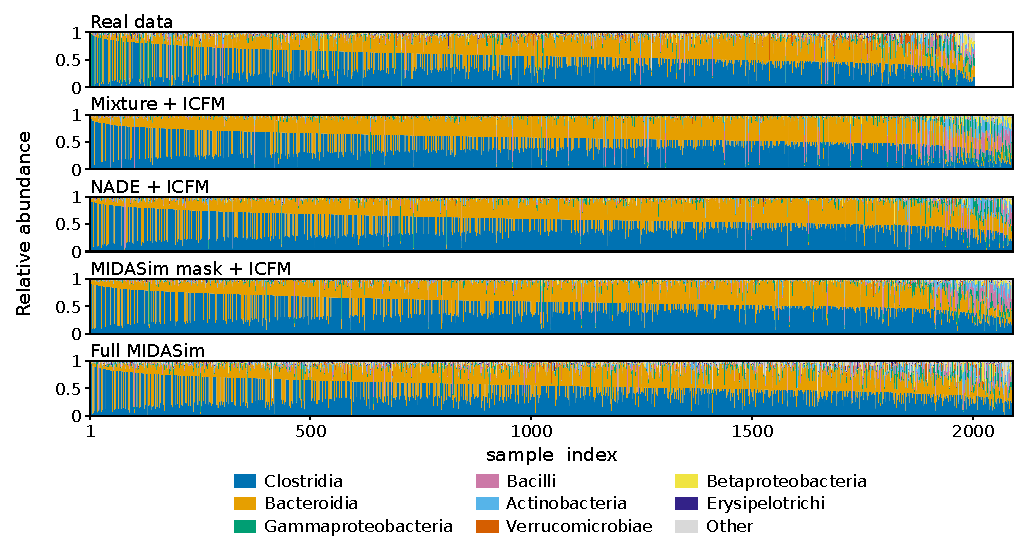
\includegraphics[width=6.8in]{results/AGP/four_generator_class_abundance_compact_20261026/class_relative_abundance_compact.pdf}
  \caption{Class-level relative abundance in real assessment data ($n=2{,}002$) and four generators ($n=2{,}089$ each). The eight classes with the highest mean abundance in the real assessment data are shown separately; the remaining 40 classes are summed as Other. All observations are retained, independently sorted within each source by decreasing largest-class abundance in the original 48-class compositions, before aggregation. Horizontal ranks are not matched observations. This descriptive view compares broad composition patterns; visual similarity alone does not establish distributional agreement. See Supplementary Fig.~\ref{fig:agp-class-abundance-full} for the full 48-class view.}
  \label{fig:agp-class-abundance-compact}
\end{figure*}

% Add this figure to the supplement to resolve the caption reference.
\begin{figure*}[p]
  \centering
  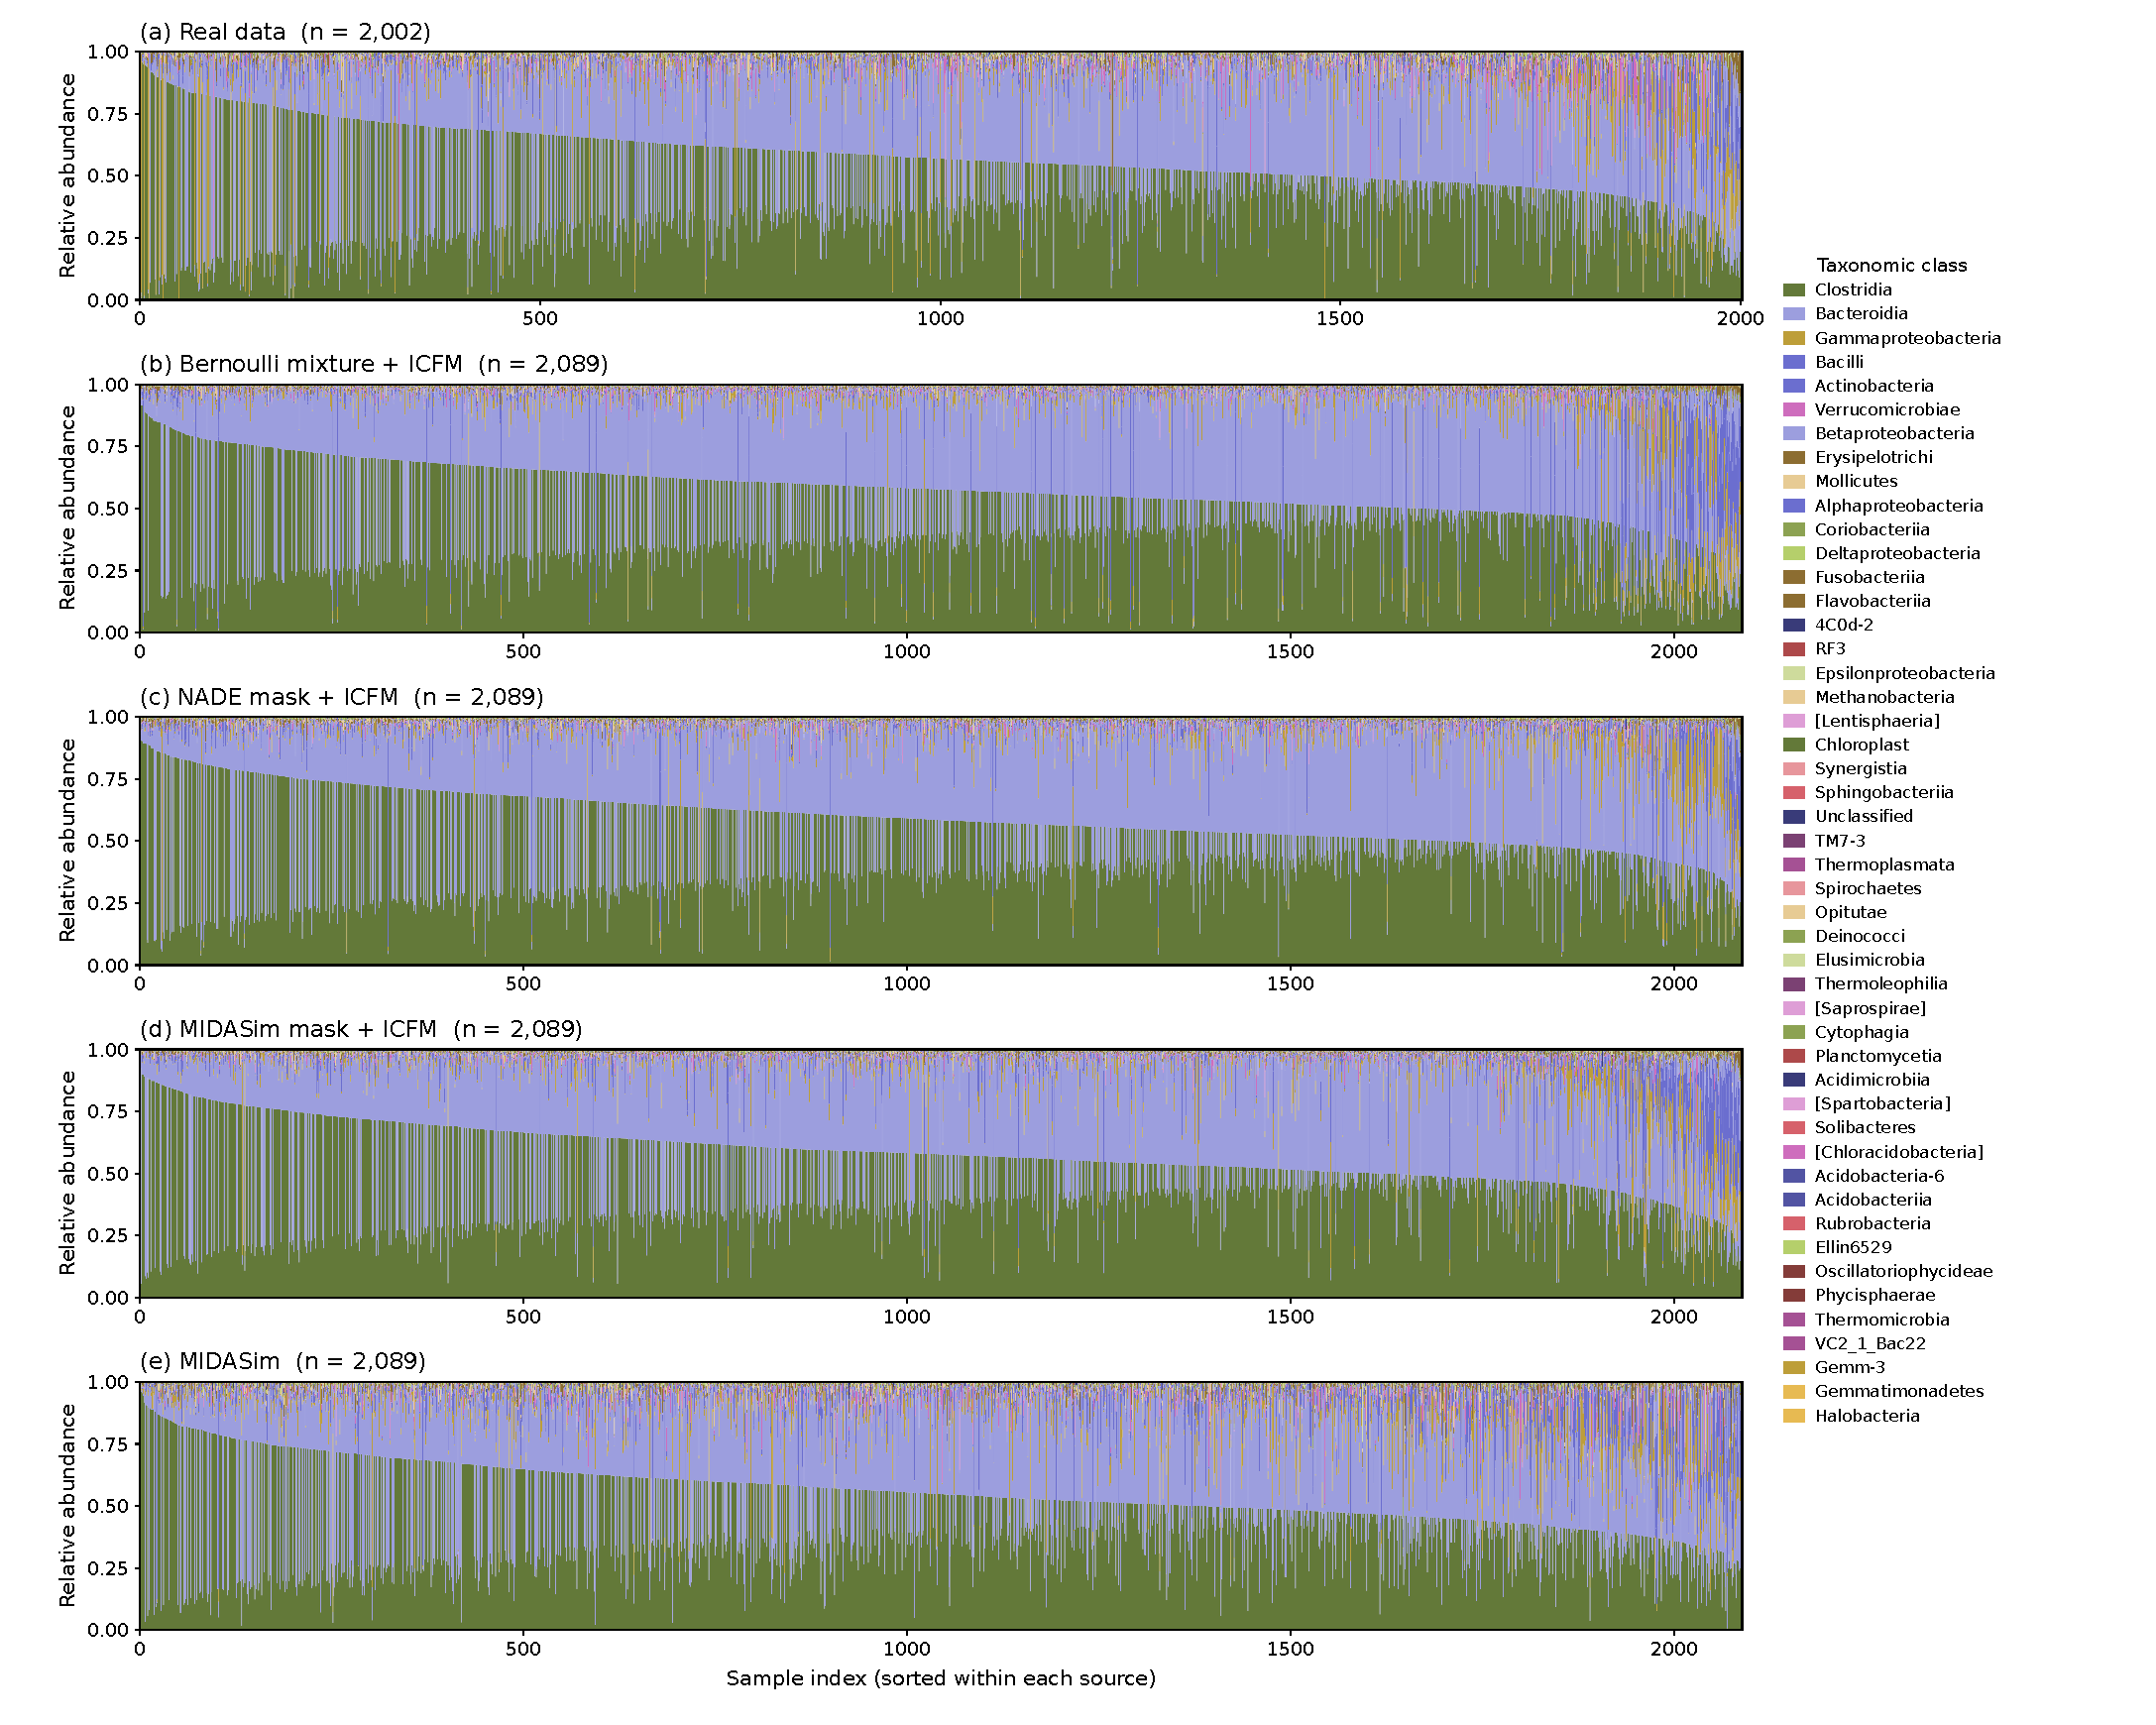
\includegraphics[width=\textwidth]{results/AGP/four_generator_class_abundance_20261022/class_relative_abundance.pdf}
  \caption{Full 48-class relative abundances for the same assessment observations, with the same independent within-source sorting as Fig.~\ref{fig:agp-class-abundance-compact}.}
  \label{fig:agp-class-abundance-full}
\end{figure*}
